\chapter{Background}

\section{Remote Attestation}

\paragraph*{}
RA is a method to prove certain properties of a system to a remote verifier. This is achieved by collecting evidence on the attested system and combining it into a report. Based on this the remote verifier should be able to draw conclusions about the desired properties. An example of such property is the integrity of the execution control flow of a process, which could also be generalized to the correct behavior of a process. It is a very difficult task to provide sufficient evidence to allow the remote verifier to prove this property. In this case for instance it is not sufficient to only check the integrity of the executable code of a process, because the process can behave differently from what is expected due to its data structures being tampered with.

\paragraph*{}
The prover (in other words the system that is attested by the verifier) requires certain abilities to correctly and securely gather evidence about itself. First of all, a trusted base enforcing an isolation mechanism is needed to avoid the evidence collecting process is tampered with. This isolation will make sure that the attestation can be executed, even when the target is unreliable due to the presence of malicious code or a compromised rich OS. Another important characteristic of the prover is the ability to gather evidence about desired properties of the system. This is often achieved by measuring certain aspects of the system, for instance, hashing a code page to allow the hash digest to be compared with the original to prove the integrity of that code page. The measurements need to be structured to allow the verifier to draw conclusions from them. Finally, the prover also needs to provide some sort of proof that the attestation report is trustworthy because the verifier relies on the authenticity of the information it receives.

\paragraph*{}
The verifier requests an attestation report from the prover when he desires to check the trustworthiness of the device. This report ideally consists of fresh and securely obtained information from the prover. The freshness is important because the evidence can in the best case only prove the trustworthiness of the device at the time the measurements were taken. Securely acquiring these measurements is also important to make sure that an adversary is not able to forge a false report to make it look like the device can be trusted while it has been compromised. Based on this information the verifier should be able to identify the state in which the prover is currently situated. The perceived state of the device can then be investigated by the verifier to determine whether the state is secure, whether it is expected or known and, finally, based on these findings, whether the verifier trusts the state of the prover and therefore the prover itself. These decisions are referred to as attestations. It is not unusual for a verifier to keep track of past attestations of a prover and use this history for more elaborate investigations.

\subsection*{Exemplary techniques}

\paragraph*{}
Integrity Measurement Architecture (IMA) \cite{IMA} implements attestation by measuring the code of programs before running them on the target. The prover is responsible for measuring the executable code pages of a process, for instance, by hashing them when the program is loaded into Random Access Memory (RAM) for execution. After all hash digests have been obtained, they need to be sent to the verifier which is required to have access to a database containing a mapping between the executable code pages of all the possible programs that can run on the prover, and their hash digest. The verifier can check whether the program's code has been modified, by comparing the newly calculated digests with the ones in its database. There is not much recent work that specifically mentions IMA, as it is often combined with other techniques or used in very specific use cases. In one paper \cite{DuanJialiang2020IMBo}, for instance, Intel Secure Guard eXtension (SGX) is used to assess code integrity (along with other aspects) of a running Virtual Machine (VM). A very similar paper \cite{KucabMichal2021Raai} describes the method to measure the code integrity (and dynamic characteristics) in a TEE provided by ARM TrustZone. According to \cite{AlamMasoom2012Aoer}, IMA is inflexible and static. On top of that, it is perceived as a very limited solution, \cite{AnkergardSigurdFrejJoelJorgensen2021Ssra} claims similar shortcomings of the reflection method \cite{SpinellisDiomidis2000Raam} which is very similar to IMA. First of all, it is inflexible or static because, if new software is introduced or software is updated, the verifier needs to update its mapping because the hash digests will certainly change. This is rather complex to manage because not all provers update at the same time. Some measurements will need to be compared to the old value, and some to the new one. Furthermore, it is not known how long this old value should be kept for attestation purposes. IMA is seen as limited because there are a variety of ways a program can misbehave without the code base being tampered with. One example of such misbehavior without the code base changing is the well-known attacks related to buffer overflows and return-oriented programming.

\paragraph*{}
Attestation on program execution goes beyond merely measuring the integrity of the executable code pages, it measures the dynamic behavior of the process. \cite{GuLiang2008Raop} proposes to observe the system calls the program makes to verify whether it adheres to the permitted control flow. This is achieved by introducing hooks on the system calls to allow the attestation procedure to intercept them. During this interception of the system call, its parameters and its time of arrival are all analyzed and afterwards stored to provide it to the verifier later. Based on the Abstract Syntax Tree (AST) and the Program Dependency Graph (PDG), the verifier should be able to verify whether a certain system call was possible. If it can correctly identify the state in which the attested program was. Although this method is a big improvement, there are still weaknesses. For example, the granularity of a system call might not give enough details about the behavior of the system. Furthermore, there is more to the behavior than the system calls alone. Many similar solutions that focus on the dynamic behavior of code have been proposed, all with their weaknesses and shortcomings. 
RIPTE \cite{QinYu2020RRIP} combines dynamic measurement and encrypts return addresses with a Physically Unclonable Function (PUF) key and it can protect software integrity at runtime. \cite{AliToqeer2017Daio} uses machine learning algorithms to verify the dynamic behavior of the prover. \cite{BaHaihe2017RMAf} provides runtime measurement and RA for Java bytecode integrity to prevent the Java Virtual Machine (JVM) from being bypassed.

\paragraph*{}
As mentioned earlier when describing IMA, different techniques are often combined to protect against a wider variety of vulnerabilities. Model-based Behavior Attestation (MBA) was proposed by \cite{AlamMasoom2008Mba}, which is again mentioned by the same researchers in their analysis of existing techniques \cite{AlamMasoom2012Aoer}, on which these exemplary techniques are based. The platform is expected to enforce a certain security model, or have its submodules enforce a certain security model. This division helps to precisely identify the behavior of each module, but it also makes sure the high-level behavior policy does not need to be made too general. This behavior policy dictates constraints and conditions which need to be adhered to by the prover. Finally, the enforcement behavior is compared to the expected behavior to check the trustworthiness of the prover. These behavior policies consist of certain properties that the module possesses. It is still very hard to map configurations of the platform to certain properties, but it does provide lots of flexibility in terms of attestation. \cite{MuhlbergJanTobias2016LaFT} also combines a variety of approaches to attest trust of IoT devices and implements multiple modules that attest certain platform properties based on different measurements. Some of these properties are OS data structures, available resources, event occurrence and event timing.  

\section{Trusted Execution Environment}

\paragraph*{}
Based on the papers of the Trusted Computing Group (TCG) \cite{TCG} and Confidential Computing Consortium (CCC) \cite{CCC}, a TEE can be defined as the following. A TEE is a standardized isolation environment for SoCs that provides a high level of assurance in terms of data integrity, data confidentiality and code integrity. This isolation is enforced by hardware architecture and the boot sequence which uses a hardware RoT, making it highly robust against software and probing attacks. Code running in the TEE and using protected resources (known as Trusted Applications (TA)) is cryptographically verified prior to execution, leading to high integrity assurance. On top of this, it is also common for a TEE to provide RA functionalities that prove its trustworthiness for third parties.

\begin{figure}[h]
\centering
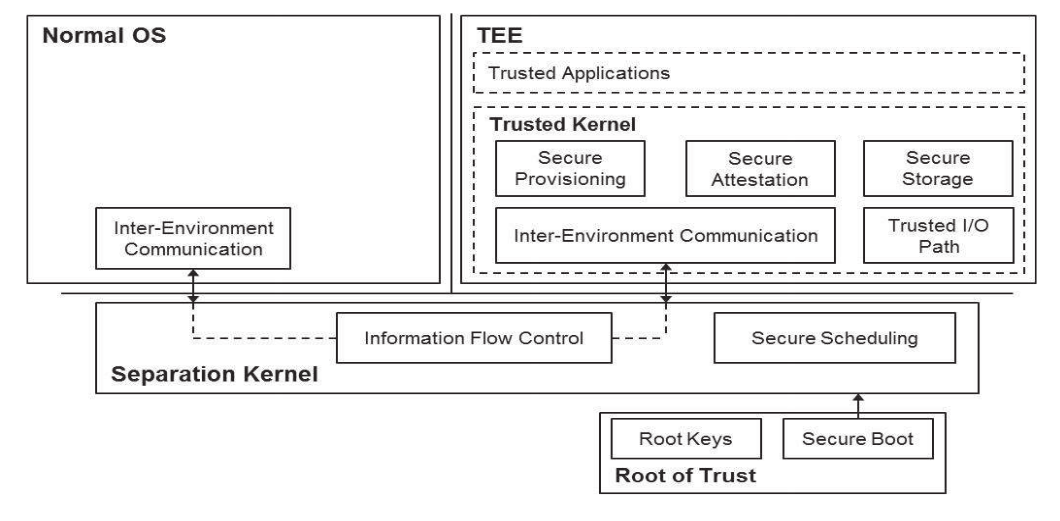
\includegraphics[width=\textwidth]{TEE_structure}
\caption{Trusted Execution Environment structure (Decomposition)}
\caption*{Source: \cite{SabtMohamed2015TEEW}}
\label{TEE}
\end{figure}

\paragraph*{}
In image \ref{TEE} from \cite{SabtMohamed2015TEEW}, the different software modules in a common TEE realization are shown. Each of these components has its responsibility and fulfills its own specific duty to guarantee the security of the TEE. 

\paragraph*{}
The secure boot makes sure the device starts up in a known state. This is achieved by verifying that the integrity of the loaded code is intact. This booting process often consists of multiple stages where the system is bootstrapped by first running the boot loader, which calls the secondary program loader, which in turn starts the SW and so on. During this process each stage decrypts the code of the next one; when the code is loaded into memory the current stage checks the integrity of the next one by checking a signature or comparing the hash digest. After the current booting phase has finished and the verification of the next phase was successful, the following phase gets control and starts executing. Since the secure boot starts from the RoT and checks the integrity of all intermediate steps before continuing, a Chain of Trust (CoT) is constructed. This CoT ends when the SW or in general the TEE has been given control. Afterwards the Normal World (NW), along with the rich OS, will receive control and here the trust is lost due to the uncertainty of the rich OS containing security vulnerabilities. This RoT is often implemented using some trusted hardware component, for instance, a Secure Cryptographic Unit (SCU) \cite{MATSUMOTOTsutomu2021SCUa} or a Trusted Platform Module (TPM) \cite{FotiadisGeorgios2021RAfS}, or finally, using a PUF \cite{ZhaoShijun2021RoRo}.

\paragraph*{}
The separation kernel has multiple responsibilities, which is logical because it is the coordinator between the Rich Execution Environment (REE) and the TEE. Secure scheduling is the first important aspect to watch over, because a balanced distribution of time slices for each environment needs to be assured. This scheduler is often implemented preemptively to avoid the TEE from affecting the responsiveness of the rich OS. Furthermore, inter-environment communication is very crucial. A strict interface is defined to enable the TEE to communicate with the rest of the system. Communication is indispensable because the TEE cannot provide any added value when it is not able to receive input or produce output. Communication also introduces a lot of threats like message overloading, control data corruption and so on. These dangers can be minimized by implementing a standardized communication mechanism like the GlobalPlatform TEE Client API \cite{TEEClientAPI}. These interfaces have been thoroughly tested and worked on by many people and they guarantee reliability in terms of memory and time isolation, providing protection of communication structures and minimum overhead by avoiding unnecessary data copies and context switches. Despite all the effort that has gone into these APIs, flaws can still arise when they are put into practice. In a paper from our University \cite{VanBulckJo2019AToT}, several sanitization vulnerabilities were found, in another paper \cite{GuoPengfei2021RoAT}, cache vulnerabilities based on the ARM TrustZone cache architecture are explained, and finally, BOOMERANG \cite{Machiry2017BOOMERANGET}, which enables NW user programs to abuse the TEE and gain control over the rich OS.

\paragraph*{}
The trusted kernel is responsible for key features that the TEE provides. This kernel is the Trusted Computing Base (TCB) of the TEE, which means that the security relies on the correctness of the code and the absence of security vulnerabilities in it. Some of these key features are secure memory and trusted I/O, which are important to allow the TEE to be used in a secure manner. Secure memory ensures confidentiality, integrity and freshness of stored data. The trusted I/O protects the authenticity and confidentiality of communication between TEE and peripherals. Besides these general security functionalities, the TAs also reside in the TEE. A TA can be developed by a third party that wishes to utilize the secure and trusted functionality of the TEE kernel, or to protect its application from the rich OS, or both. A TA can be called by applications in the REE with a very constrained interface to avoid as many threats as possible. During this execution, the TA has similar privileges to other code running in the TEE. The TEE often enforces multiple levels of privilege, a TA is less privileged than a trusted kernel process, similar to how a user application has fewer privileges than a rich OS process.

\subsection*{Trust}

\paragraph*{}
Trust is a core aspect of a TEE, therefore, it is important to establish a notion of what it means to trust something. Trust is a firm belief in the reliability, truth, or ability of someone or something. In computer sciences, there are multiple types of trust with respect to devices. Besides there being differences in types of trust, it is also important to be able to quantify this trust to compare different types and levels of trust. The Common Criteria (CC) \cite{trust} are an international standard that specifies seven evaluation assurance levels, where higher levels envelop all requirements of the preceding levels.

\paragraph*{}
First of all, there is static trust: this type of trust is evaluated only once and assumed to never change during the lifetime of the device. The analysis often takes place before the device is deployed to ensure no malicious code or security vulnerabilities can be introduced by an adversary. For this type of trust, the evaluation assurance levels from the CC are often used. Dynamic trust, on the other hand, is based on the state of the system and this state changes continuously. In this latter case, the trust needs to be measured continuously to have an up to date understanding of it. Generally, a TEE has both types of trust: it needs static trust for the code running inside the TEE (TAs and the trusted kernel), but it also needs static trust when booting up which is provided by the RoT. During execution the TEE of course needs to maintain its level of trust, and this needs to be checked with the methods for measuring dynamic trust.

\paragraph*{}
To perform these measurements, a trusted module or device is required, because if the trust level of an object is measured with an untrusted tool, these measurements can never be fully trusted. With this analogy in mind, it can be derived that a RoT as mentioned earlier is required to start a CoT up to the measuring component. In a CoT the trust from one intermediate component is transferred to the next, because this following component does not have any inherent trust. Components are not inherently trusted because if the environment in which they are started is malicious, it is very hard if not impossible to guarantee the reliability or security of this component. Transferring trust from one component to the next is done by each component checking the next one on authenticity, integrity and reliability, and based on this evaluation, the next component is given control to do its task. 

\section{ARM TrustZone}

\paragraph*{}
ARM TrustZone \cite{TrustZone} implements the TEE on the processor level, which means it runs below the hypervisor or OS \cite{PintoSandro2019DATA}. This approach divides the system into two main partitions, namely the NW and the SW. The processor executes either in the NW or in the SW, as these environments are completely isolated in terms of hardware. The SW is more privileged to make sure a maliciously behaving NW can not damage the SW. The partition between these worlds gives rise to new and better security solutions for applications running on these types of SoCs. An example of this is a reliable on/off switch of device peripherals \cite{LentzMatthew2018SATM}. Fidelius \cite{EskandarianSaba2018FPUS} protects sensitive user input from a malicious browser, MIPE \cite{ChangRui2017Mapm} protects sensitive data and code in the SW and is formally proven by the B method, and finally, Komodo \cite{FerraiuoloAndrew2017KUvt} attempts to provide similar security guarantees as Intel SGX on ARM TrustZone.  

\paragraph*{}
While providing additional security, ARM TrustZone only has a minimal impact on performance due to it being implemented on hardware \cite{AmacherJulien2019Otpo} \cite{HuaZhichao2021Tpcf}. ARM TrustZone makes sure that there is a TEE available with capabilities like secure memory, trusted I/O and many others. The trusted kernel is responsible for making partitions of the memory only accessible to the SW, which should then be able to provide secure data storage services to NW applications. Secure data storage is necessary to make sure that data from one application cannot be read or modified by another one. Trusted I/O paths, on the other hand, allow the user application to request I/O features from the SW instead of the rich OS. Because these connections go through the SW, the rich OS is not able to inspect or modify the data that is transmitted to the I/O peripheral, which is important in cases where an adversary has gained control over the rich OS.

\subsection*{Implementation}

\begin{figure}[h]
\centering
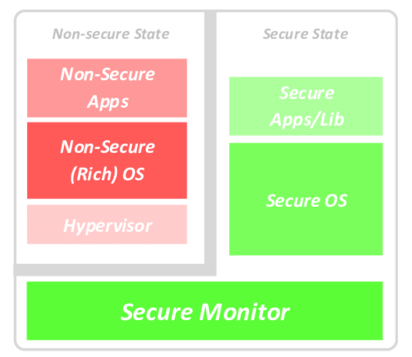
\includegraphics[width=0.5\textwidth]{ARMTrustZone}
\caption{ARM TrustZone architecture (Decomposition)}
\caption*{Source: \cite{PintoSandro2019DATA}}
\label{TZ}
\end{figure}

\paragraph*{}
The NW and the SW are the two main environments in which the processor will be executing code. In image \ref{TZ}, these environments are called non-secure state and secure state respectively. The NW shelters the rich OS (like Linux). It is mainly due to the size of these operating systems that they cannot be trusted to run in the SW. The risk of including implementation bugs that introduce security risks, is too high. Also, user-level applications run in the NW, for access to peripherals they rely on the rich OS and, depending on the service, the rich OS relies on the SW. Some services can also be requested from the user application directly to the SW. The SW is where the trusted kernel runs. The implementation of this component is kept very minimal and needs to be designed and implemented very securely to avoid vulnerabilities.

\paragraph*{}
The secure monitor, which can be seen at the bottom of figure \ref{TZ}, is responsible for keeping these two execution environments isolated from each other. The NS-bit is an additional bit that flows through the entire pipeline and can be read from the Secure Configuration Register (SCR) to identify the world in which the operation is being executed. The processor has a third state, which is the monitor state. This is necessary to preserve and sanitize the processor state when making transitions between NW and SW states. The new privileged instruction Secure Monitor Call (SMC) allows both worlds to request a world switch, the monitor state will make sure this is handled correctly. The only other way of getting into the monitor state is with exceptions or interrupts from the SW.

\paragraph*{}
This secure monitor of course needs to have an overview of which environment is allowed to access certain memory regions, this is nicely described in \cite{PintoSandro2019DATA}. For this, the TrustZone Address Space Controller (TZASC) is introduced. The TZASC can be used to configure specific memory regions as secure or non-secure, such that applications running in the SW can access memory regions associated with the NW, but not the other way around. Making these partitions is also performed by the TZASC, which is made available through a programming interface only available from within the SW. A similar approach is taken for off-chip Read-Only Memory (ROM) and Static Random Access Memory (SRAM), which is implemented using the TrustZone Memory Adapter (TZMA). Whether these components are available or not and how finely grained the memory can be partitioned, depends on the SoC, because they are optional and configurable. Besides the memory, there are also the peripherals which need to be monitored, and depending on the execution environment, access needs to be denied. The TrustZone Protection Controller (TZPC) is in the first place used to restrict certain peripherals from worlds, for instance, to only allow the SW to access them. It also extends the Generic Interrupt Controller (GIC) with support for prioritized interrupts from secure and non-secure sources. This prioritization is important to avoid Denial of Service (DoS) attacks on the SW.

\section{PinePhone}

\paragraph*{}
Many smartphone manufacturers use ARM SoC for their devices. Thanks to the introduction of ARM TrustZone, these companies are extending their security solutions with these TEE capabilities. An example of this is Samsung KNOX \cite{KNOX}, but large companies like Google are also able to increase their security guarantees using these functionalities, for instance, Android KeyStore \cite{KeyStore}. The drawback of this is that the security solutions of these major companies are not made public. What is even worse, is that these devices cannot be used to experiment with the TEE. On the one hand, this is logical because additional software running in the SW could compromise the security of the entire device, but on the other hand, having these large companies decide which software may run on the device and which cannot, brings about a very closed and exclusive community. To provide the academic world and hardware security enthusiasts with an open platform on which these ARM TrustZone features are available, PinePhone developed a smartphone device for which all hardware developments are open to the public, and they also take into account the development ideas of their community \cite{PinePhone}. Not only the hardware that is used is made open source, but the main operating system is Linux \cite{PineSoft} which enables the user to control every nook and cranny of the device. A large community working with the PinePhone also helps to solve issues, or find related solutions when working with such a device.

\section{OP-TEE}

\begin{figure}[h]
\centering
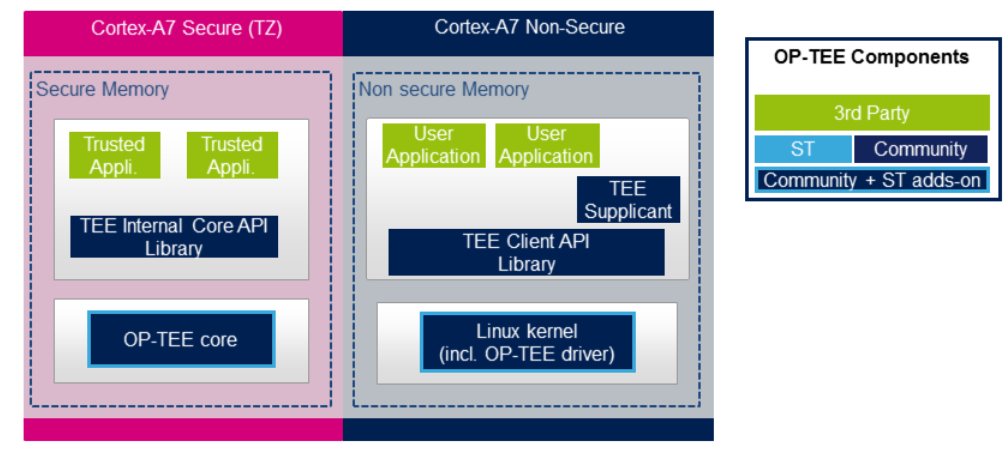
\includegraphics[width=\textwidth]{OPTEE_structure}
\caption{OP-TEE structure (Process)}
\caption*{Source: \cite{OP-TEE_structure}}
\label{OPTEE}
\end{figure}

\paragraph*{}
OP-TEE stands for Open Portable TEE \cite{OP-TEE}: it is an open-source implementation with ARM TrustZone in mind, but it applies to other realizations of TEEs as well. It implements two Application Programming Interfaces (APIs) defined in the GlobalPlatform API specifications: TEE internal core API v1.1 \cite{TEECoreAPI} is exposed to trusted applications, and TEE Client API v1.0 \cite{TEEClientAPI} defines how to communicate with a TEE. The main design principles for OP-TEE are isolation, small footprint and portability, as the name describes. As is required for a TEE, it provides isolation from the non-secure OS and shields the TAs from each other. The TEE should also remain small enough to reside in the On-Chip Memory (OCM) of the ARM-based devices. OP-TEE aims at being easily pluggable to different architectures, and has to support various setups like multiple OSs or TEEs. 

\paragraph*{}
As can be seen in figure \ref{OPTEE}, OP-TEE allows for third parties to write TAs that can enjoy the added security guarantees the SW has to offer. Despite these trusted applications residing inside the SW, they are not able to compromise the security guarantees of other TAs running on the same platform. This fact is very important, especially when advocating an open platform where software of different stakeholders can run simultaneously. For the academic community, this is also a very interesting architecture, because the OP-TEE core is open source, meaning it can be extended. These extensions can easily be implemented by creating a Pseudo Trusted Application (PTA), which is similar to a TA but with the same privileges as the trusted kernel. Caution is required, because software bugs in the OP-TEE kernel could introduce security vulnerabilities in the TEE, which defies the added security it provides. Nonetheless, it is very important to experiment with these features and produce research explaining the best practices, pitfalls and innovative ways in which the TEE can be extended.

\section{Secure boot, trusted boot and remote attestation for ARM TrustZone-based IoT Nodes \cite{LingZhen2021Sbtb}}

\paragraph*{}
The paper \cite{LingZhen2021Sbtb} about secure boot, trusted boot and RA attempts to enforce system integrity on ARM TrustZone based IoT devices. To achieve this, they need to guarantee system integrity during load time, and during runtime. The load time integrity is made possible with what they call a hybrid booting approach, which consists of a secure boot up to the SW and proceeds with a trusted boot for the rest of the system. To achieve runtime integrity a RA scheme is used, which checks the integrity of executable memory pages of processes running in the NW. With this approach, they endeavor to protect IoT devices against malicious pre-installed programs or malware injection during runtime.

\subsection*{System overview}

\paragraph*{}
The threat model assumes that attackers have physical access to the IoT device and can launch a wide variety of attacks, like software and OS attacks. They are able to tamper with the images of the SW and NW (including that of the OS) before the device is booted up. The adversary can also inject malware into the NW during runtime and tamper with the NW applications. Bus snooping, cold boot and cache side-channel attacks are not considered, even though these are possible with physical access. Only the security of the text section of programs is considered. On the other hand, it is assumed that programs that reside in On-Chip Read Only Memory (OCROM) are secure, because this type of memory is hard to tamper with. Lastly, the execution environment of the SW and the RA server are assumed to be trustworthy and secure.

\paragraph*{}
The solution that is proposed uses a hybrid booting method to ensure the load time integrity of the system and RA to ensure the runtime integrity. Secure boot is used to load everything up to the kernel of the SW. This provides strong guarantees that the SW starts in a secure and known state. The NW is booted with what is called trusted boot, which uses attestation to provide proof of the integrity of the image that is being started. Before the control is given to the rich OS, its image is measured and after it has started, it should send this to the RA server to verify the measurement. The RA service is implemented in the SW. The memory pages of the rich OS are periodically measured using a hash function. The hash digest is encrypted by an attestation key and sent to the RA server for verification.

\subsection*{Hybrid booting}

\begin{figure}[h]
\centering
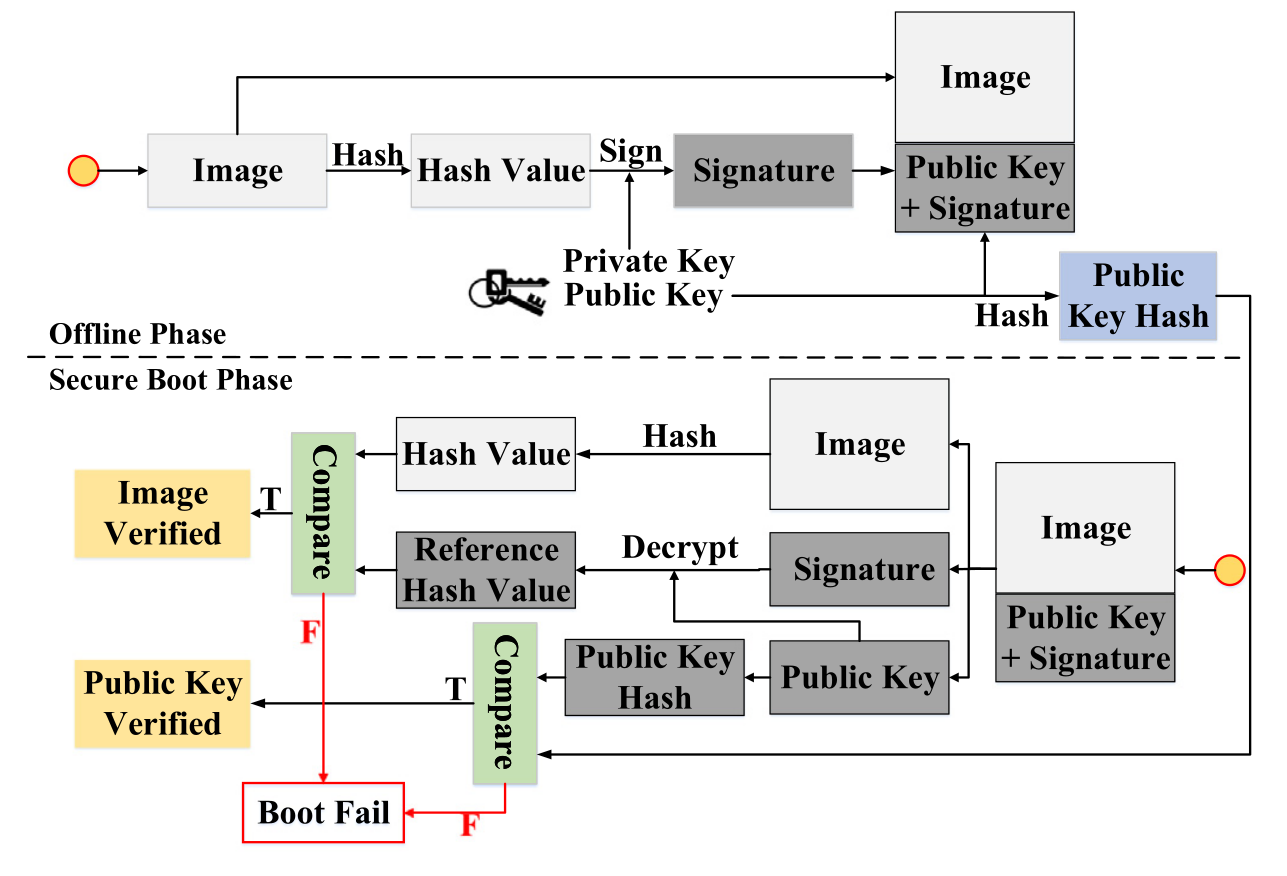
\includegraphics[width=\textwidth]{secure_boot}
\caption{Secure boot process sequence}
\caption*{Source: \cite{LingZhen2021Sbtb}}
\label{secureboot}
\end{figure}

\paragraph*{}
The setup of secure boot starts with a RoT, which in this case is achieved by using the OCROM and eFuse of the IoT device. The first-stage bootloader is encrypted with a private key and stored on the OCROM to verify the integrity during the boot phase as can be seen in figure \ref{secureboot}. The hash of the public key is stored in the eFuse to verify its integrity during the boot phase. The images of the second-stage bootloader and secure kernel are measured and signed before deploying the device. These measurements and signatures are stored in the flash memory while the hash of the public key of the secondary bootloader is stored in the eFuse. The hash of the public key of the trusted kernel is stored in the secondary bootloader to achieve an incremental chain.

\paragraph*{}
The secure boot phase starts with the first-stage bootloader which locates the second-stage bootloader, the public key and its signature. Secondly, the first-stage bootloader calculates the hash of the public key and verifies the integrity of the public key. After successful verification, it uses the public key to obtain the measurement result for the second-stage bootloader. Finally, the first-stage bootloader calculates the hash of the second-stage bootloader and verifies its correctness. The second-stage bootloader does this entire process for the secure kernel to complete the secure boot phase.

\begin{figure}[h]
\centering
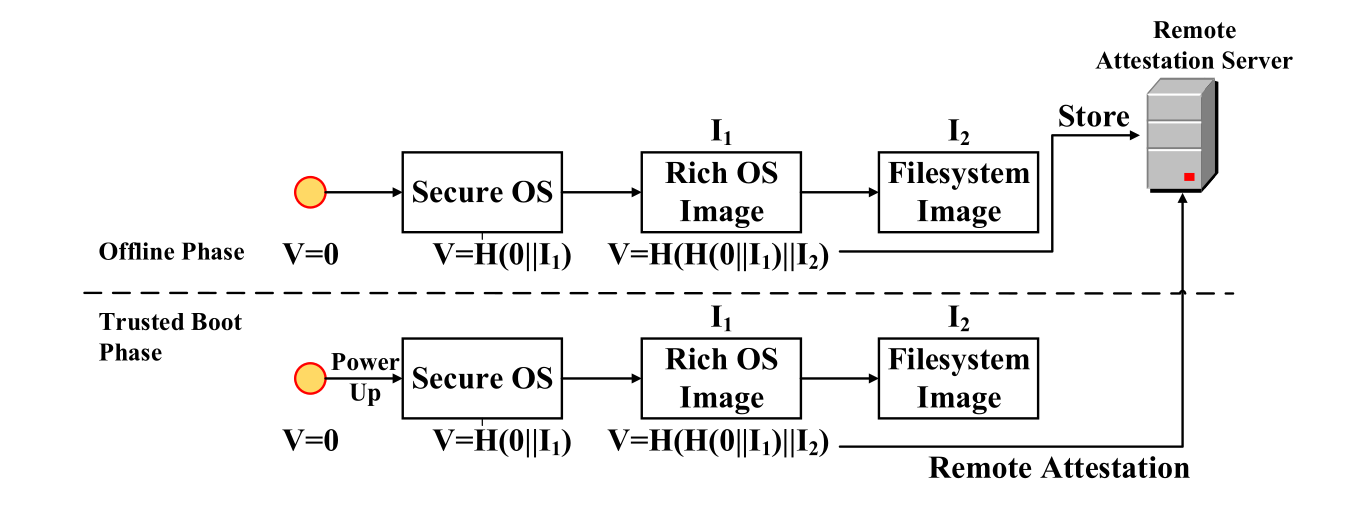
\includegraphics[width=\textwidth]{trusted_boot}
\caption{Trusted boot process sequence}
\caption*{Source: \cite{LingZhen2021Sbtb}}
\label{trustedboot}
\end{figure}

\paragraph*{}
Trusted boot is set up by producing a hash chain: the image of the secure OS is hashed first and concatenated with the image of the rich OS, and hashed and concatenated with the image of the file system, and hashed again. This final hash value is stored in the RA server, during runtime this hash value will need to be securely sent to the RA server. To achieve secrecy a symmetric key is used (the attestation key): storing this in the IoT device is not trivial, so this is solved with the following method. The Cryptographic Acceleration and Assurance Module (CAAM) is used to execute cryptographic functions in a secure environment. This module is used to generate a 256-bit blob key, which is used to encrypt the attestation key that has been agreed on with the RA server. A Message Authentication Code (MAC) is calculated from the attestation key to ensure its integrity. The blob key is itself encrypted with a Blob Key Encryption Key (BKEK), which is derived from the Master Key (MK) by the CAAM. The MK is stored in Secure Non-Volatile Storage (SNVS), which is assumed to be secure by default. To prevent the NW from ever gaining access to the attestation key, the CAAM is configured to be only accessible from the SW using the TZPC, as discussed earlier.

\paragraph*{}
The trusted boot phase starts with the NW attestation client application establishing a Transport Layer Security (TLS) connection with the RA server, and requesting a nonce. The measurement TA restores the attestation key from the blob, using the CAAM. The TA measures the rich OS and filesystem images, appends the nonce to the final hash value and encrypts this combination with the attestation key. The encrypted text is put in shared memory to allow the client application to send it to the RA server. On the RA server, the cyphertext is decrypted and verified to check for integrity violations and replay attacks.

\subsection*{Page-based attestation}

\paragraph*{}
The idea is to measure the code segments of the programs in the NW on the IoT device. It is assumed that this code base does not change in the lifetime of the device. The SW is trusted but the NW is still vulnerable to attackers, therefore attesting the code in the NW would increase the security of the applications running in the NW. The measurement is done on pages of 4 KB at a time so programs will have multiple tuples of the form \textit{\{process-name, page-hash\}} which will later be used to verify the integrity of the process. The first measurement is done before deploying the IoT device, and the results are stored on the RA server to be able to compare the future measurements with. 

\begin{figure}[h]
\centering
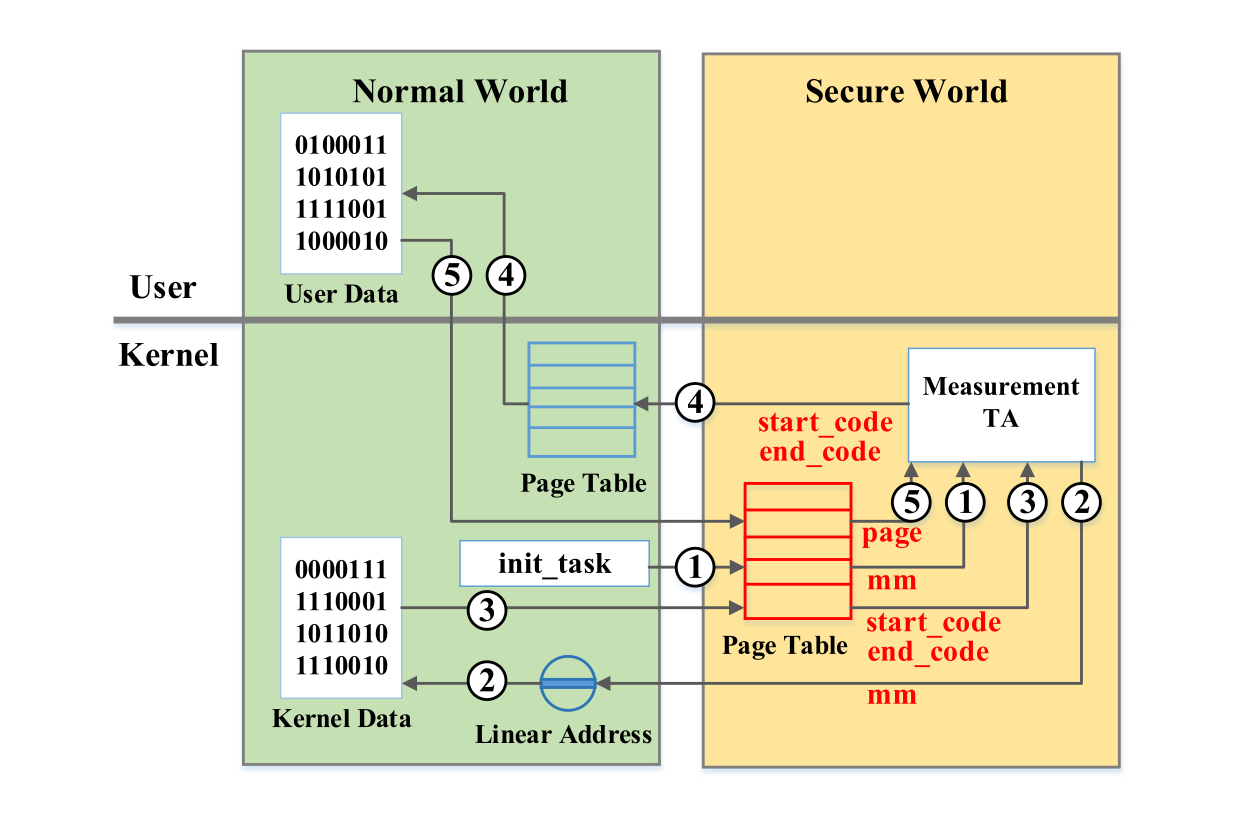
\includegraphics[width=\textwidth]{process_measurement}
\caption{Process measurement sequence}
\caption*{Source: \cite{LingZhen2021Sbtb}}
\label{processmeasurement}
\end{figure}

\paragraph*{}
Process integrity measurement starts with the kernel of the NW providing the \textit{task\_struct} of the initial process \textit{init\_proc} to the measurement TA (1). The \textit{task\_struct} is a data structure containing all information about a process, for instance, the virtual address where it resides (2). This address is sent back to the kernel of the NW, because only there it can be investigated to find out about the boundaries of this memory region (3). The fourth step (4) is to search for this memory region in the kernel of the NW from where the process can be accessed. Next (5), the executable code pages of the NW process are sent to the SW, which is achieved by storing them in shared memory space. Based on the \textit{init\_proc}, the TA is able to iterate over all processes and measure their code pages. These \textit{task\_struct}s have the structure of a doubly-linked list, so it enables the TA to find all processes during the measurements. 

\paragraph*{}
Process integrity attestation uses the measurement of the process integrity measurement stage. First, the IoT device requests a nonce from the RA server, with which a TLS connection is established. The measurement TA encrypts the measurement results concatenated with the nonce, using the attestation key. Based on the assumption that the attestation key is kept secure, and the execution control flow of the measurement TA is secure, also guarantees the freshness of the measurements. If any of those two assumptions were violated the attestation response could be forged by an adversary, because that the nonce is only concatenated with the hash digest. The measurements of the processes are encrypted individually, meaning that a set of cypher texts is sent to the RA server. The RA server decrypts the measurements of the processes and checks whether integrity violations can be found, which means that there is new software or old software has been modified.

\subsection*{Evaluation} 

\paragraph*{}
The effectiveness of the secure boot process is measured by whether the secure boot phase can detect any violations against the integrity of the images, the signatures or the public key. All of these inconsistencies are exposed by the secure boot process correctly. For the trusted boot the focus lies on whether the RA server can identify an abnormal system status. This is the case because NW programs can still be executed, but the RA server will verify the system state. The process integrity attestation is tested by tampering with existing programs and inserting additional programs. Both cases are picked up on by the attestation. 

\paragraph*{}
Performance of the boot procedures is measured by comparing the mean time of 30 iterations with secure and trusted boot, and 30 iterations without it. The secure boot adds little overhead on the second-stage bootloader, while the trusted boot almost doubles the time it takes for the secure kernel to boot, which comes down to a little over a second being added. The main reason why the secure kernel takes this long is that the image of the filesystem and rich OS is rather large and takes some time to measure. The overhead of the measurement TA and the attestation CA is measured by calling rich OS services, while these modules are running and with them disabled. The overhead these modules introduce lies between $-0.55\%$ and $+0.67\%$.

\paragraph*{}
Security analysis is executed on the hybrid booting approach and the page-based process attestation. In the booting method a CoT is constructed from the RoT residing in the eFuse and OCROM. A successful secure boot ensures that the SW can be seen as the secure base from which the NW can be booted. If the NW image is tampered with, the RA server will pick up on this threat. The execution of the measurement TA and the results it generates are both secure because of the isolation in the SW. The results pass through the NW, but they are encrypted at this stage; the encryption key is also securely stored in the SW, giving the NW no opportunity to get hold of the information. The main drawback of this approach is that the method relies on the rich OS to access the paging structure and process management kernel objects.

\paragraph*{}
In \cite{LingZhen2021Sbtb} it is correctly mentioned that the proposed solution does not detect self hiding malware, for example, transient rootkits. There are, however, more shortcomings when the solution is investigated. The attestation method is not sufficient to detect all software attacks due to it not checking the integrity of key aspects of the system like data structures, system calls, etc. The same reasoning can be applied to OS and firmware attacks. The fact that they state: \textit{\enquote{We only consider the security of the code section of a program}} is honest, but alarming nonetheless.  